\chapter{Installation and Getting Help}
\label{cha:installation}

Figure~\ref{fig:install:choices} provides a guide to select the
appropriate method for installing PyLith.  Installation of PyLith on a
desktop or laptop machine is, in most cases, very easy. Binary
packages have been created for Linux and Mac OS X (Darwin) platforms. For
Windows 10 users, we recommend installing the Windows Subsystem for
Linux and using the Linux binary (see instructions in
Section~\ref{sec:install:windows}). You can also run PyLith
inside a Docker container, which provides a virtual Linux environment
on any platform that Docker supports, including Linux, Mac OS X, and
Windows. Installation of PyLith on other operating systems -- or
installation on a cluster -- requires building the software from the
source code, which can be difficult for inexperienced users. We have
created a small utility called PyLith Installer that makes installing
PyLith and all of its dependencies from source much easier.

\begin{figure}[htbp]
  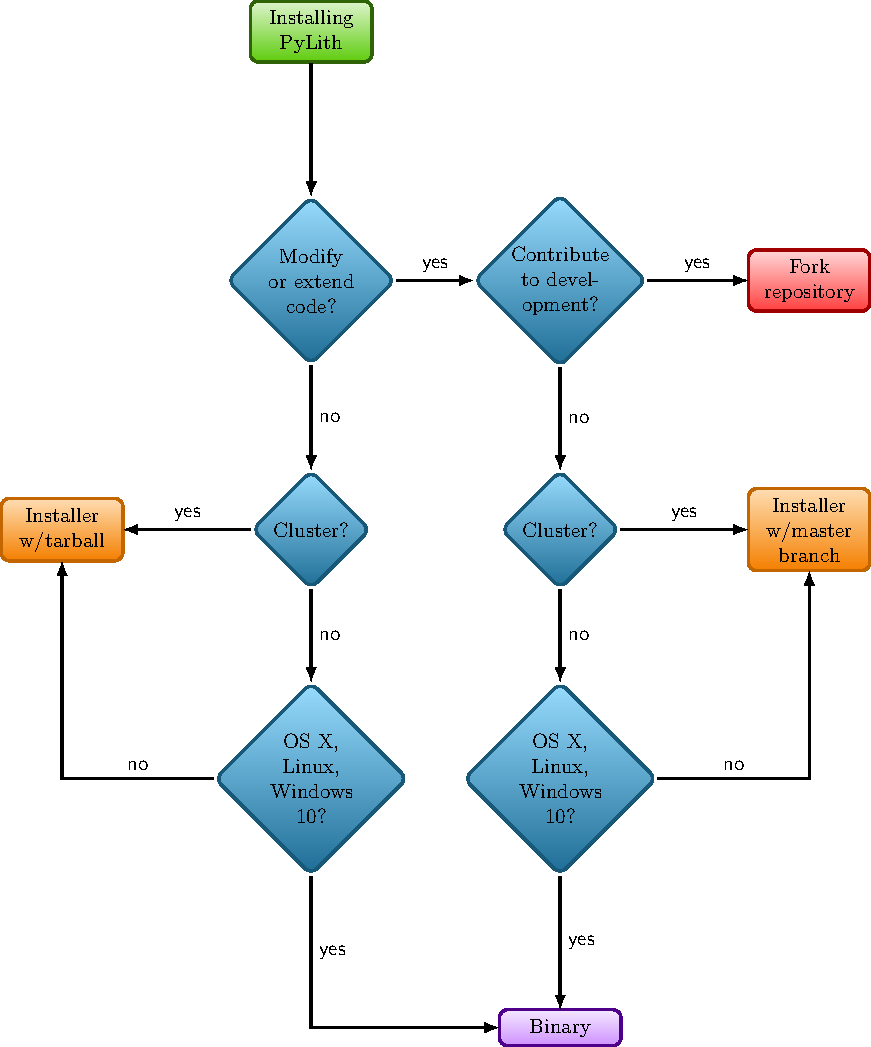
\includegraphics[scale=0.8]{install/figs/installchoices} 
  \caption{Guide for selecting the appropriate installation choice
  based on a hardware and intended use. The installation options are
  discussed in more detail in the following sections.}
\label{fig:install:choices} 
\end{figure}

Help for installing and using PyLith is available from both a CIG
mailing list and the GitHub issue tracking system
\url{https://github.com/geodynamics/pylith/issues}. See
Section~\vref{sec:help} for more information.

\section{Installation of Binary Executable}

The binaries are intended for users running on laptops or desktop
computers (as opposed to clusters). The binaries contain the compilers
and header files, so users wishing to extend the code can still use
the binary and do not need to build PyLith and its dependencies from
source. See Chapter~\vref{cha:extending} for more information on
extending PyLith.

Binary executables are available for Linux (glibc 2.12 and later) and
Mac OS X (Intel 10.10 and later) from the PyLith web page
\url{geodynamics.org/cig/software/packages/short/pylith/}. Users
running Windows 10 build 14316 and later can install a Linux bash
environment and use the PyLith binary for Linux (see
Section~\vref{sec:install:windows} for more information).

\tip{On Linux systems you can check which version of glibc you have by
  running \filename{ldd --version}}.

\tip{On Darwin systems running OS X, you can check the operating
  system version by clicking on the Apple icon and \menu{About this Mac}.}

\subsection{Linux and Max OS X (Darwin)}
\begin{enumerate}
\item Open a terminal window and change to the directory where you
  want to place the distribution.
  \begin{shell}
$ cd  $HOME
$ mkdir pylith
$ cd pylith
  \end{shell}
\item Download the Linux or Mac OS X (Darwin) tarball from the PyLith
  web page \url{geodynamics.org/cig/software/packages/short/pylith/},
  and save it to the desired location, e.g., \filename{\$HOME/pylith}.
\item Unpack the tarball.
  \begin{shell}
# Linux 32-bit
$ tar -xzf pylith-2.2.1-linux-i686.tgz
# Linux 64-bit
$ tar -xzf pylith-2.2.1-linux-x86_64.tgz
# Mac OS X
$ tar -xzf pylith-2.2.1-darwin-10.11.6.tgz
  \end{shell}
\item Set environment variables. The provided \filename{setup.sh}
  script only works if you are using bash shell. If you are using a
  different shell, you will need to alter how the environment
  variables are set in \filename{setup.sh}.
  \begin{shell}
$ source setup.sh
  \end{shell}
\end{enumerate}

\warning{The binary distribution contains PyLith and all of its
  dependencies. If you have any of this software already installed on
  your system, you need to be careful in setting up your environment
  so that preexisting software does not conflict with the PyLith
  binary. By default the \filename{setup.sh} script will prepend to
  the PATH and PYTHONPATH (for Darwin and Linux) and LD\_LIBRARY\_PATH
  (for Linux) environment variables. This will prevent most
  conflicts.}

\warning{The PyLith binary distribution for {\bf Darwin} systems is
  built using the system clang compiler suite and the system
  Python. {\bf This means the system Python must be in your path to
    use the PyLith binary executable}; ensure \filename{/bin} and
  \filename{/usr/bin} are at the beginning of the PATH environment
  variable, which is done automatically if you use the
  \filename{setup.sh} script. {\bf This condition is often violated if
    you have Python installed from Anaconda, HomeBrew, MacPorts,
    etc. and set the PATH variable in your bash configuration file.}}

\subsection{Windows 10}
\label{sec:install:windows}

PyLith is developed within the Unix/Linux framework, and we do not
provide a native PyLith binary distribution for Windows. The preferred
approach to installing PyLith on a computer running Windows 10 is to
enable use of a Linux subsystem. This permits use of the PyLith Linux
x86\_64 binary within the bash environment.

To enable the Linux subsystem on Windows 10 build 14316 and later
(users running an earlier Windows build should use the PyLith Docker
container):
\begin{enumerate}
\item Go to \menu{Settings} $\rightarrow$ \menu{Security}.
\item Under \menu{For developers} select \menu{Developer mode}. This
  step should not be required for Windows build 16215 and later.
\item Go to \menu{Control Panel} $\rightarrow$ \menu{Programs}
  $\rightarrow$ \menu{Turn Windows Features On or Off}.
\item Enable \menu{Windows Subsystem for Linux} and click \menu{OK}.
\item Restart the computer.
\item Go to \menu{Start} $\rightarrow$ \menu{bash}. You will be
  prompted to download "Bash on Ubuntu on Windows" from the Windows
  Store. Create a user account and password for the bash environment.
\item Install the PyLith Linux x86 binary within the bash environment
  following the instructions for installing the PyLith binary for
  Linux. You will run PyLith within the bash environment just like you
  would for a Linux operating system.
\end{enumerate}

\subsection{Extending PyLith and/or Integrating Other Software Into PyLith}
\newfeature{v.2.2.0}

We have constructed the binary package so that you can extend PyLith
and/or build additional software for integration with PyLith using the
binary distribution.

\begin{description}
\item[Darwin] The binary package includes the header files for PyLith
  and all of its dependencies. Use the clang compiler and Python
  provided with the operating system. You will need to install XTools.
\item[Linux] The binary package includes the GNU compilers, Python, as
  well as header files for PyLith and all of its dependencies.
\end{description}

\tip{We encourage anyone extending PyLith to fork the PyLith
  repository and build from source using the PyLith Installer Utility
  to facilitate contributing these features back into the CIG
  repository via pull requests.}

\section{Installation of PyLith Docker Container}

As an alternative to installing a binary package, we provide a Docker
container for running PyLith in a self-contained virtual
environment. Docker containers provide a self-contained virtual
environment that are a smaller, simpler alternative to a virtual
machine. The PyLith Docker container provides a Debian Linux
environment with a pre-built PyLith executable, vim text editor,
iceweasel (GNU version of Firefox) web-browser, and the matplotlib
Python module.

\tip{In nearly all cases, installing a PyLith binary provides easier
  integration with mesh generation and post-processing tools, so
  binaries are the preferred approach to using the PyLith Docker
  container. This installation method targets users running Windows
  versions earlier than Windows 10 build 14316.}

\subsection{Setup (first time only)}

\begin{enumerate}
\item Install Docker (See \url{https://www.docker.com/products/docker})
\item Create a container to store persistent user data\\
  This container, called pylith-data, will hold a directory where all
  your user data can be stored for use with PyLith within Docker. The
  data can persist for different versions of PyLith; that is, you can
  update to a newer version of PyLith and your user data will still
  be available. This directory is not directly accessible from your
  host computer. However, you can copy files to/from your host filesystem
  using ``docker cp'' (see below).
\end{enumerate}
\begin{shell}[]
# Create the container
$ docker create --name pylith-data geodynamics/pylith-data
# Run the docker container and copy examples to the persistent storage.
$ docker run -ti --volumes-from pylith-data geodynamics/pylith
# This next command is run WITHIN the docker container.  
$ cp -R $HOME/pylith-VERSION/examples $HOME/data
\end{shell}

\subsection{Run Unix shell within Docker to use PyLith.}

To run the container with a text only interface:
\begin{shell}
$ docker run -ti --volumes-from pylith-data geodynamics/pylith
\end{shell}

To run the container and allow display of windows on the host computer
(requires that X-Windows be installed):
\begin{shell}
# Darwin: Allow X connections
$ xhost +YOUR_IP_ADDRESS; DISPLAY=YOUR_IP_ADDRESS:0
# Linux: Allow X connections
$ xhost +local:root
# For Linux and Darwin, continue with the follow lines.
$ XSOCK=/tmp/.X11-unix
$ docker run -ti --volumes-from pylith-data \
    -e DISPLAY=$DISPLAY -v $XSOCK:$XSOCK geodynamics/pylith
\end{shell}

In addition to a minimalist Debian Linux distribution and PyLith and
all of its dependencies, the container includes the following useful
utilities:
\begin{description}
\item[vim] Lightweight text editor
\item[matplotlib] Python plotting module
\item[iceweasel] GNU version of Firefox
\end{description}

\important{We do not yet include ParaView due to difficulties
  associated with setting up rendering on the host display outside the
  container. You will need to copy the output files to your host
  machine to view them in ParaView as described later.}

\subsubsection{Using Docker containers}
\begin{itemize}
\item To ``pause'' a container: \texttt{Control-p Control-q}
\item To attach to a ``paused'' or ``running'' container.
  \begin{shell}
# Get the container id.
$ docker ps
# Attach to the container
$ docker attach CONTAINER_ID
  \end{shell}
\item To restart an existing container after it exited.
  \begin{shell}
# Get the container id.
$ docker ps -a
# Start and then attach to the container
$ docker run CONTAINER_ID
$ docker attach CONTAINER_ID
  \end{shell}
\end{itemize}

\subsection{Copy data to/from persistent storage volume.}

These commands are run on the local host outside the container, not
inside the Docker container. These commands are used to move files
from your host machine into the PyLith Docker container and vice
versa. For example, you will generate your mesh on the host, copy the
mesh file into the Docker container, run PyLith within the container,
and then copy the output files to the host to display in ParaView.

\begin{shell}
# Copy data FROM persistent storage volume TO local host
$ docker cp pylith-data:/data/pylith-user/PATH/FILENAME LOCAL_PATH
# Copy data FROM local host TO persistent storage volume
$ docker cp LOCAL_PATH pylith-data:/data/pylith-user/PATH/
\end{shell}


\subsection{Docker Quick Reference}
\begin{shell}
# List local docker images.
$ docker images
# List all docker containers.
$ docker ps -a
# List running docker containers.
$ docker ps
# Remove docker container
$ docker rm CONTAINER_ID
# Remove docker image
$ docker rmi IMAGE_ID
\end{shell}

\section{Installation from Source}

PyLith depends on a number of other packages (see Figure
\vref{fig:pylith-dependencies}).  This complicates building the
software from the source code. In many cases some of the packages
required by PyLith are available as binary packages. On the one hand,
using the binary packages for the dependencies removes the burden of
configuring, building, and installing these dependencies, but that can
come with its own host of complications if consistent compiler and
configuration settings are not used across all of the packages on
which PyLith depends. This is usually not an issue with Linux
distributions, such as Fedora, Ubuntu, and Debian that have good
quality control; it can be an issue with Darwin package managers, such
as Fink, MacPorts, and Homebrew, where there is limited enforcement of
consistency across packages. Nevertheless, PyLith can be built on most
systems provided the instructions are followed carefully. PyLith is
developed and tested on Linux and Mac OS X.

A small utility, PyLith Installer, removes most of the obstacles in
building PyLith and its dependencies from source. For each package
this utility downloads the source code, configures it, builds it, and
installs it. This insures that the versions of the dependencies are
consistent with PyLith and that the proper configure arguments are
used. The minimum requirements for using the PyLith installer are a C
compiler, \filename{tar}, and \filename{wget} or \filename{curl}.
Detailed instructions for how to install PyLith using the installer
are included in the installer distribution, which is available from
the PyLith web page
\url{geodynamics.org/cig/software/packages/short/pylith/}.


\section{Verifying PyLith is Installed Correctly}

The easiest way to verify that PyLith has been installed correctly is
to run one or more of the examples supplied with the binary and source
code. In the binary distribution, the examples are located in
\filename{src/pylith-\pylithVersionNumber/examples} while in the source distribution,
they are located in \texttt{pylith-\pylithVersionNumber/examples}. Chapter
\vref{cha:examples} discusses how to run and visualize the results
for the examples. To run the example discussed in Section
\vref{sec:example:3dhex8-static}:
\begin{shell}
$ cd examples/3d/hex8
$ pylith step01.cfg
# A bunch of stuff will be written to stdout. The last few lines should be:  
WARNING! There are options you set that were not used!
WARNING! could be spelling mistake, etc!
Option left: name:-snes_atol value: 1.0e-9
Option left: name:-snes_converged_reason (no value)
Option left: name:-snes_error_if_not_converged (no value)
Option left: name:-snes_linesearch_monitor (no value)
Option left: name:-snes_max_it value: 100
Option left: name:-snes_monitor (no value)
Option left: name:-snes_rtol value: 1.0e-10
\end{shell}
If you run PyLith in a directory without any input, you will get the
error message:
\begin{shell}
$ pylith
 >> {default}::
 -- pyre.inventory(error)
 -- meshimporter.meshioascii.filename <- ''
 -- Filename for ASCII input mesh not specified.
    To test PyLith, run an example as discussed in the manual.
 >> {default}::
 -- pyre.inventory(error)
 -- timedependent.homogeneous.elasticisotropic3d.label <- ''
 -- Descriptive label for material not specified.
 >> {default}::
 -- pyre.inventory(error)
 -- timedependent.homogeneous.elasticisotropic3d.simpledb.label <- ''
 -- Descriptive label for spatial database not specified.
 >> {default}::
 -- pyre.inventory(error)
 -- timedependent.homogeneous.elasticisotropic3d.simpledb.simpleioascii.filename <- ''
 -- Filename for spatial database not specified.
pylithapp: configuration error(s)
\end{shell}
This indicates that a number of default settings must be set in order
to run PyLith, including setting the filename for the finite-element
mesh.


\section{Configuration on a Cluster}

If you are installing PyLith on a cluster with a batch system, you can
configure Pyre such that the \filename{pylith} command automatically
submits jobs to the batch queue. Pyre contains support for the LSF,
PBS, SGE, and Globus batch systems.

The command to submit a batch job depends upon the particular batch
system used. Further, the command used in a batch script to launch an
MPI program varies from one cluster to the next. This command can vary
between two clusters, even if the clusters use the same batch system!
On some systems, \filename{mpirun} is invoked directly from the batch
script. On others, a special wrapper is used instead.

Properly configured, Pyre can handle job submissions automatically,
insulating users from the details of the batch system and the site
configuration. This feature has the most value when the system
administrator installs a global Pyre configuration file on the cluster
(under \filename{/etc/pythia-0.8}), for the benefit of all users and
all Pyre-based applications.


\subsection{Launchers and Schedulers}
\label{sec:launchers:schedulers}

If you have used one of the batch systems, you will know that the
batch system requires you to write a script to launch a
job. Fortunately, launching a parallel PyLith job is simplified by
Pyre's \texttt{launcher} and \facility{scheduler} facilities. Many
properties associated with \facility{launcher} and \facility{scheduler}
are pertinent to the cluster you are on, and are best customized in a
configuration file. Your personal PyLith configuration file
(\filename{\$HOME/.pyre/pylithapp/pylithapp.cfg}) is suitable
for this purpose. On a cluster, the ideal setup is to install a
system-wide configuration file under \filename{/etc/pythia-0.8}, for the
benefit of all users.

Pyre's \facility{scheduler} facility is used to specify the type of
batch system you are using (if any):
\begin{cfg}
<h>[pylithapp]</h>
# The valid values for scheduler are 'lsf", 'pbs', 'globus', and 'none.
<f>scheduler</f> = lsf
# Pyre's launcher facility is used to specify the MPI implementation.
# The valid values for launcher include 'mpich' and 'lam-mpi'.
<f>launcher</f> = mpich
\end{cfg}

You may find the 'dry' option useful while debugging the \facility{launcher}
and \facility{scheduler} configuration. This option causes PyLith to perform a ``dry run,'' dumping the
batch script or mpirun command to the console, instead of actually submitting it for
execution (the output is only meaningful if you're using a batch system).
\begin{shell}
# Display the bash script that would be submitted.
$ pylith --scheduler.dry
# Display the mpirun command.
$ pylith --launcher.dry
\end{shell}

\subsection{Running without a Batch System}

On a cluster without a batch system, you need to explicitly specify
the machines on which the job will run. Supposing the machines on your
cluster are named n001, n002, \ldots, etc., but you want to run the
job on machines n001, n003, n004, and n005 (maybe n002 is down for the
moment). To run an example, create a file named
\filename{mymachines.cfg} which specifies the machines to use:
\begin{cfg}
<h>[pylithapp.launcher]</h>
<p>nodegen</p> = n%03d
<p>nodelist</p> = [1,3-5]
\end{cfg}
The \property{nodegen} property is a printf-style format string, used
in conjunction with \property{nodelist} to generate the list of machine
names. The \texttt{nodelist} property is a comma-separated list of
machine names in square brackets.

Now, invoke the following:
\begin{shell}
$ pylith example.cfg mymachines.cfg
\end{shell}
This strategy gives you the flexibility to create an assortment of
\filename{cfg} files (with one \filename{cfg} file for each machine
list) which can be easily paired with different parameter files.

If your machine list does not change often, you may find it more convenient
to specify default values for \property{nodegen} and \property{nodelist}
in \filename{\$HOME/.pyre/pylithapp/pylithapp.cfg} (which
is read automatically). Then, you can run any simulation with no additional
arguments:
\begin{shell}
$ pylith example.cfg
\end{shell}

\warning{This assumes your machine list has enough nodes for the
  simulation in question.}

You will notice that a machine file \filename{mpirun.nodes} is generated.
It will contain a list of the nodes where PyLith has run.

\subsection{Using a Batch System}

Many clusters use some implementation of a PBS (e.g., TORQUE/Maui)
or LSF batch system. The examples below illustrate use of some of
the more important settings. You may need to make use of more options
or adjust these to submit jobs on various cluster. These settings
are usually placed in \filename{\$HOME/.pyre/pylithapp/pylithapp.cfg}
or in a system-wide configuration file. They can be overridden on
the command line, where one typically specifies the number of compute
nodes and number of processes per compute node, the job name, and
the allotted time for the job:
\begin{shell}
$ pylith example1.cfg \
    --job.queue=debug \
    --job.name=example1 \
    --job.stdout=example1.log \
    --job.stderr=example1.err \
    --job.walltime=5*minute \
    --nodes=4
\end{shell}
\important{The value for nodes is equal to the number of compute nodes
  times the number of processes (usually the number of cores)
  requested per compute node. Specifying the number of processes per
  compute node depends on the batch system. For more information on
  configuring Pyre for your batch system, see CIG's Pythia page
  \url{geodynamics.org/cig/software/packages/cs/pythia}.}


\subsubsection{LSF Batch System}
\begin{cfg}
<h>[pylithapp]</h>
<f>scheduler</f> = lsf    ; the type of batch system

<h>[pylithapp.lsf]</h>
<p>bsub-options</p> = [-a mpich_gm]    ; special options for 'bsub'

<h>[pylithapp.launcher]</h>
<p>command</p> = mpirun.lsf    ; 'mpirun' command to use on our cluster

<h>[pylithapp.job]</h>
<p>queue</p> = normal    ; default queue for jobs
\end{cfg}

\subsubsection{PBS Batch System}
\begin{cfg}
<h>[pylithapp]</h>
<f>scheduler</f> = pbs     ; the type of batch system

<h>[pylithapp.pbs]</h>
<p>shell</p> = /bin/bash     ; submit the job using a bash shell script

# Export all environment variables to the batch job
# Send email to johndoe@mydomain.org when the job begins, ends, or aborts
<p>qsub-options</p> = -V -m bea -M johndoe@mydomain.org

<h>[pylithapp.launcher]</h>
<p>command</p> = mpirun -np ${nodes} -machinefile ${PBS_NODEFILE}
\end{cfg}
For most PBS batch systems you can specify N processes per compute
node via the command line argument \commandline{-{}-scheduler.ppn=N}.

\section{Getting Help and Reporting Bugs}
\label{sec:help}

The CIG Short-Term
Crustal Dynamics Mailing List \url{cig-short@geodynamics.org} is
dedicated to CIG issues associated with short-term crustal dynamics,
including the use of PyLith. You can subscribe to the mailing list and
view messages at cig-short Mailing List
\url{geodynamics.org/cig/lists/cig-short}.

CIG uses \object{GitHub} for source control and bug tracking. If you
find a bug in PyLith, please submit a bug report to the GitHub issue
tracking system for PyLith \url{https://github.com/geodynamics/pylith/issues}.
Of course, it is helpful to first check to see if someone else already
submitted a report related to the issue; one of the CIG developers
may have posted a work around to the problem. You can reply to a current
issue by clicking on the issue title. To submit a new issue, click
on the \object{New Issue} button.


% End of file
